\newsavebox{\smlmat}
\savebox{\smlmat}{$\smm{\bullet&\bullet\\\bullet& }$}
\newsavebox{\smlmatb}
\savebox{\smlmatb}{$\smm{\bullet&\bullet\\\bullet&\bullet}$}
\newsavebox{\smlmatc}
\savebox{\smlmatc}{$\smm{\bullet&\bullet&\bullet\\ &\bullet& }$}

\chapter{Characterizations}

\begin{defn}
A \emph{walk} in a matrix~$M$ is a sequence of some of its entries, beginning in the top left corner and ending in the bottom right one. If an entry $M[i,j]$ is in the sequence, the next one is either $M[i+1,j]$ or $M[i,j+1]$. A \emph{reverse walk} in $M$ is a sequence of some of its entries, beginning in the top right corner and ending in the bottom left one. In an entry $M[i,j]$ is in the sequence, the next one is either $M[i+1,j]$ or $M[i,j-1]$.
\end{defn}

\begin{defn}
We call a binary matrix~$M$ a \emph{walking matrix} if there is a walk in $M$ such that all one-entries of $M$ are contained on the walk.
\end{defn}

\begin{defn}
For $M\in\Mat$ and $r\in[m],c\in[n]$ we say $M[r,c]$ is
\begin{itemize}
	\item \emph{top-left empty} if $M[[r-1],[c-1]]$ is an empty matrix,
	\item \emph{top-right empty} if $M[[r-1],[c+1,n]]$ is empty,
	\item \emph{bottom-left empty} if $M[[r-1],[c+1,n]]$ is empty,
	\item \emph{bottom-right empty} if $M[[r-1],[c+1,n]]$ is empty.
\end{itemize}
\end{defn}

\begin{defn}
For $M\in\Mat$ and $M'\in\{0,1\}^{m\times l}$ we define $M\rightarrow M'\in\{0,1\}^{m\times(n+l)}$ to be a matrix created by extending $M$ by adding columns of $M'$.
\end{defn}

\section{Empty rows and columns}
\label{sec:empty}

\begin{obs}
\label{obs:emptyrows}
For any $P\in\Pat$ let $P'=P\oplus_h0^{k\times1}$, and for any $M\in\Mat$ let $M'=M\oplus_h1^{m\times1}$, then $\PimM\Leftrightarrow P'\im M'$.
\end{obs}
\begin{proof}
\begin{itemize}
	\item[$\Rightarrow$] Clearly, we can map the last column of $P'$ just to the last column of $M'$ and then map $P'[[k],[l]]$ to $M'[[m],[n]]$ the same way $P$ is mapped to $M$.
	\item[$\Leftarrow$] Holds trivially, because we can take the restriction of the mapping of $P'$ to $M'$ to get a mapping of $P$ to $M$.
\end{itemize}
\end{proof}

The same proof can be used for adding an empty column as the first column or an empty row as the first or the last row. Using induction we can easily show that a pattern $P'$ is avoided by a matrix $M'$ if and only if $P$ is avoided by $M$ where $P$ is derived from $P'$ by excluding all empty leading or ending rows and columns and $M$ is derived from $M'$ by excluding the same number of leading or ending rows and columns. Therefore, when characterizing matrices avoiding a forbidden pattern, we do not need to consider patterns having empty rows or columns on their boundary.

The following theorem shows what happens when we add empty columns in between two columns of a pattern that only has two columns. The proof comes in Chapter~\ref{intervals}, where we introduce several tools useful for proving it.

\begin{thm}
\label{thm:emptymiddle}
For all $M\in\Mat$ it holds $M\in Av(P^l)\Leftrightarrow$ there exists $N\in\{0,1\}^{m\times(n-l)}$ such that $N\in Av(P)$ is inclusion maximal and $M$ is a submatrix of $N\oplus_h0^{m\times l}$ placed over $0^{m\times l}\oplus_hN$ with elementwise OR.
\end{thm}

Open questions
\begin{itemize}
	\item insertion of an empty column in between all columns of $P$
\end{itemize}

Next, we characterize matrices avoiding some small patterns. Because of the above results, we also characterize some of their generalizations and we completely omit empty lines in them. If $\PnimM$ then also $P^T\nim M^T$ and this holds for all rotations and mirrors of $P$ and $M$ and so we only mention these symmetries and do not prove all characterizations one by one.

\section{Patterns having two one-entries and their generalization}
\label{sec:2ones}
These are up to rotation and mirroring the only patterns having two one-entries and no empty lines:
$$P_1=\smm{\bullet&\bullet}\ \ \ P_2=\smm{ &\bullet\\\bullet& }$$
They can be generalized to:
$$P'_1=\smm{\bullet&\cdots&\bullet}\ \ \ P'_2=\smm{ & &\bullet\\ &\cdots& \\\bullet& & }$$

\begin{thm}
For all matrices $M$: $P_1\nim M\Leftrightarrow M$ has at most one non-empty column.
\end{thm}
\begin{proof}
\begin{itemize}
	\item[$\Leftarrow$] $M$ having at most one non-empty column does not contain $P_1$.
	\item[$\Rightarrow$] When $M$ has two columns $c_1,c_2$ having a one-entry $M[r_1,c_1],M[r_2,c_2]$ respectively, those give us a mapping of $P_1$.
\end{itemize}
\end{proof}

\begin{thm}
Let $P'_1=\{1\}^{1\times k}$. For all matrices $M$: $P'_1\nim M\Leftrightarrow M$ has at most $k-1$ non-empty columns.
\end{thm}
\begin{proof}
\begin{itemize}
	\item[$\Leftarrow$] $M$ having at most $k-1$ non-empty columns does not contain $P'_1$.
	\item[$\Rightarrow$] When $M$ has $k$ columns $c_1,c_2,\dots,c_k$ each having a one-entry $M[r_1,c_1],\\M[r_2,c_2],\dots,M[r_k,c_k]$ respectively, those give us a mapping of $P'_1$.
\end{itemize}
\end{proof}

\begin{thm}
\label{thm:walking}
For all matrices $M$: $P_2\nim M\Leftrightarrow M$ is a walking matrix.
\end{thm}
\begin{proof}
\begin{itemize}
	\item[$\Leftarrow$] a walking matrix does not contain $P_2$.
	\item[$\Rightarrow$] When $M$ is not a walking pattern then there are two one-entries that cannot be in the same walk and those give us a mapping of $P_2$.
\end{itemize}
\end{proof}

\begin{thm}
Let $P'_2\in\{0,1\}^{k\times k}$. For all matrices $M$: $P'_2\nim M\Leftrightarrow M$ contains one-entries in at most $k-1$ walks.
\end{thm}
\begin{proof}
\begin{itemize}
	\item[$\Leftarrow$] $M$ containing one-entries in at most $k-1$ walks does not contain $P'_2$.
	\item[$\Rightarrow$] When one-entries of $M$ cannot fit into $k-1$ walks, then there are $k$ one-entries where no pair can fit to a single walk and those giving us a mapping of $P'_2$.
\end{itemize}
\end{proof}

\section{Patterns having three one-entries and their generalization}
\label{sec:3ones}
These are up to rotation and mirroring the only patterns having three one-entries and no empty lines that we did not characterize so far:
$$P_3=\smm{\bullet&\bullet\\\bullet& }\ \ \ P_4=\smm{ &\bullet& \\\bullet& & \\ & &\bullet}\ \ \ P_5=\smm{\bullet& &\bullet\\ &\bullet& }\ \ \ P_6=\smm{ &\bullet&\bullet\\\bullet& & }$$

\begin{thm}
\label{thm:p31}
For all matrices $M\in\Mat$: $P_3\nim M\Leftrightarrow$ there exist a row~$r$ and a column~$c$ such that (see Figure~\ref{fig:p12})
\begin{itemize}
\item $M[[r-1],[c-1]]$ is empty,
\item $M[[r-1],[c+1,n]]$ is empty,
\item $M[[r+1,m],[c-1]]$ is empty and
\item $M[[r,m],[c,n]]$ is a walking matrix.
\end{itemize}
\end{thm}
\begin{figure}[!ht]
\centering
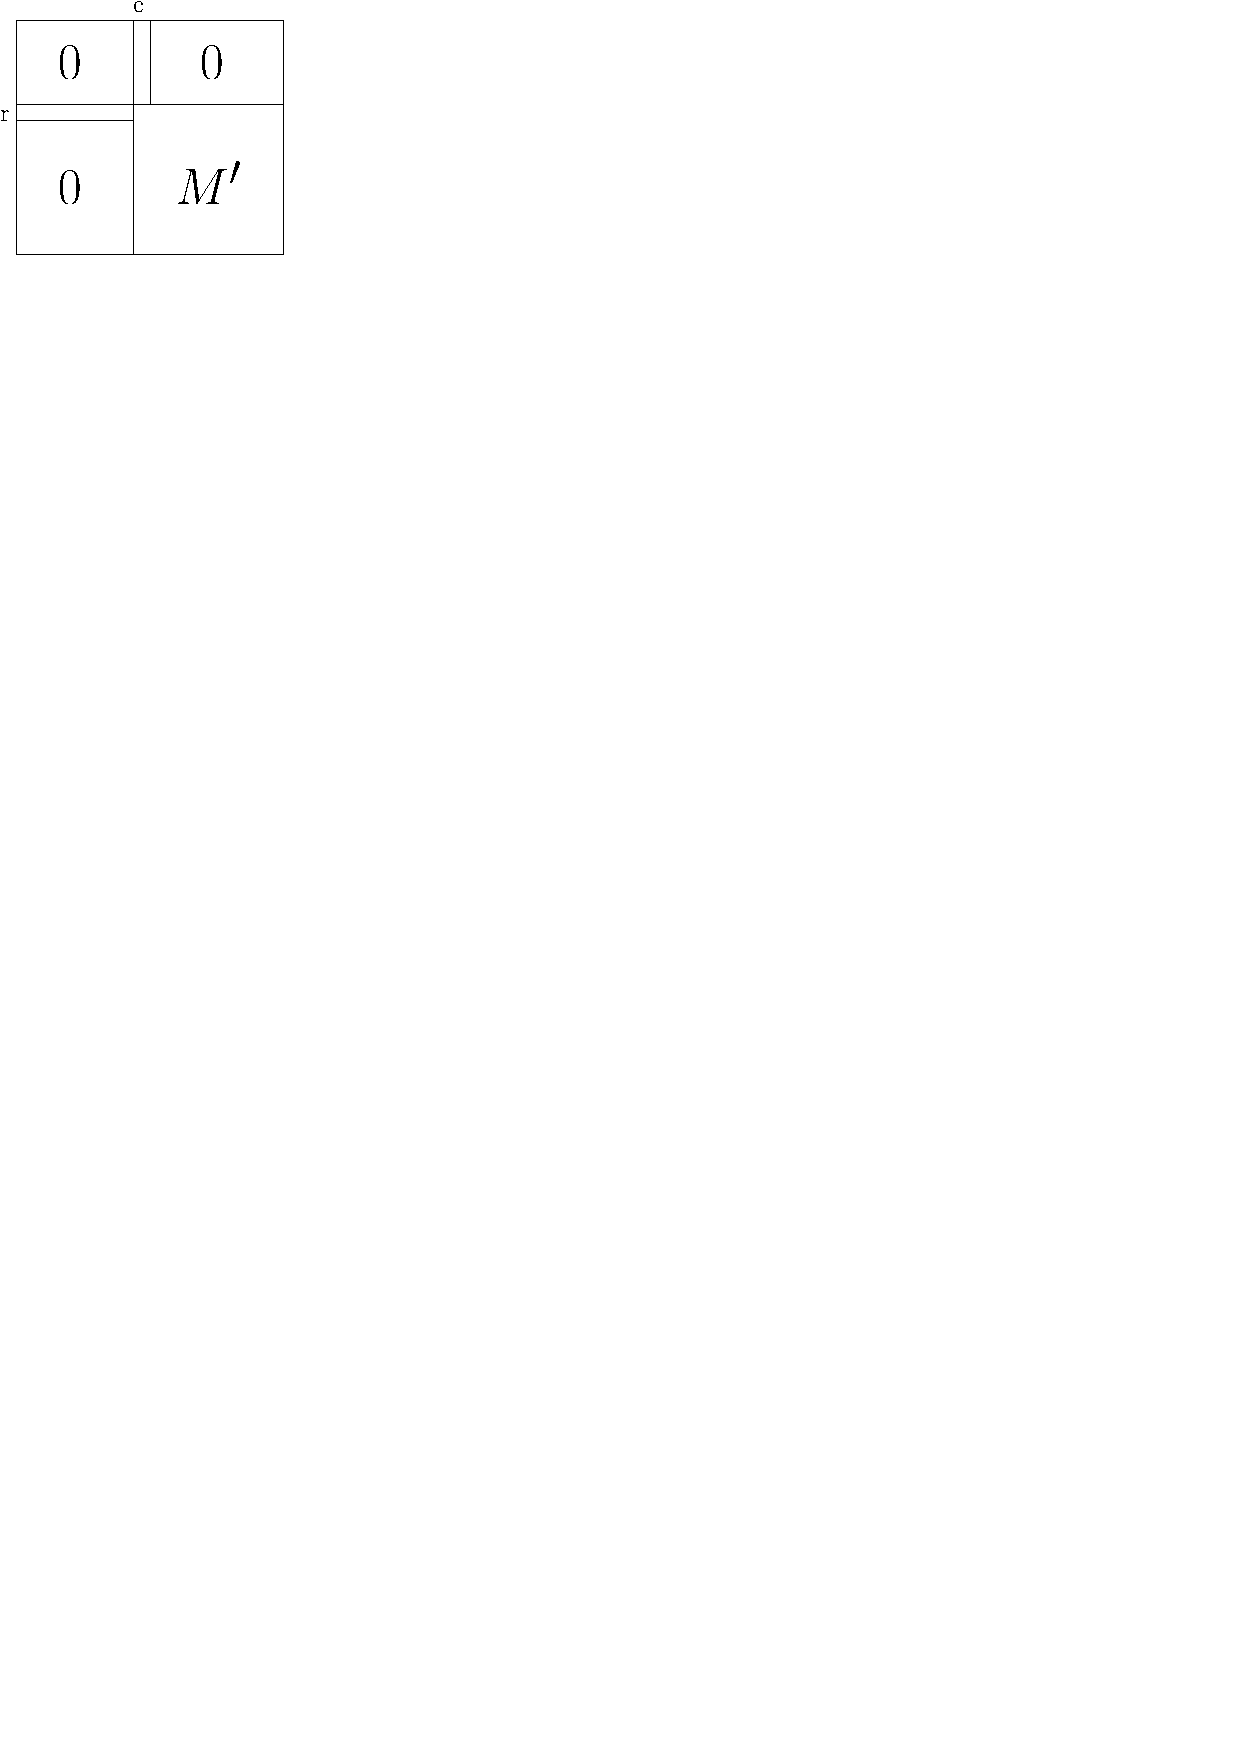
\includegraphics[width=50mm]{img/p12.pdf}
\caption{Characterization of matrices avoiding \usebox{\smlmat} as an interval minor. Matrix $M'$ is a walking matrix.}
\label{fig:p12}
\end{figure}
\begin{proof}
\begin{itemize}
	\item[$\Rightarrow$] If $M$ is a walking matrix then we set $r=c=1$. Otherwise, there are one-entries $M[r,c']$ and $M[r',c]$ such that $r'<r$ and $c'<c$. If there is a one-entry in $M[[r-1],[c-1]],\ M[[r-1],\ [c+1,n]]$ or $M[[r+1,m],[c-1]]$ then $\PimM$. If $M[[r,m],[c,n]]$ is not a walking matrix then it contains $\smm{ &\bullet\\\bullet& }$ and together with $M[r,c']$ it gives us the forbidden pattern.
	\item[$\Leftarrow$] For contradiction, assume that $M$ described in Figure~\ref{fig:p12} contains $P_3$ as an interval minor. Without loss of generality we can assume $P_3[1,1]$ is mapped to the $r$-th row. But then both $P_3[1,2]$ and $P_3[2,1]$ need to be mapped to $M'$ which is a contradiction with it being a walking matrix.
\end{itemize}
\end{proof}

\begin{thm}
For all matrices $M$: $P_4\nim M\Leftrightarrow$ for the top-left most reverse walk~$w$ in $M$ such that there are no one-entries underneath it and for every one-entry $M[r,c]$ on $w$ it holds $M[[r-1],[c-1]]$ is a walking matrix.
\end{thm}
\begin{proof}
\begin{itemize}
	\item[$\Rightarrow$] For contradiction assume there are $r,c$ such that $M[r,c]$ is a one-entry of $w$ and $M[[r-1],[c-1]]$ is not a walking matrix. It means that $\smm{ &\bullet\\\bullet& }\im M[[r-1],[c-1]]$ and together with $M[r,c]$ it gives us the forbidden pattern and a contradiction.
	\item[$\Leftarrow$] For contradiction let $P_4\im M$ and consider a mapping of $P_4$, where $P_4[3,3]$ is mapped to $M[r,c]$ and there is no other one-entry in $M[[r,m],[c,n]]$. Clearly, $M[r,c]$ cannot lie on $w$, because then $M[[r],[c]]$ is a walking matrix and so $M[r,c]$ cannot be used to map $P_4[3,3]$. So $M[r,c]$ lies above $w$ but that is a contradiction with $w$ being top-left most reverse walk in $M$ without one-entries underneath it.
\end{itemize}
\end{proof}

\begin{thm}
For all matrices $M$: $P_5\nim M\Leftrightarrow M=M_1\rightarrow M_2$ where $\smm{\bullet& \\ &\bullet}\nim M_1$ and $\smm{ &\bullet\\\bullet& }\nim M_2$.
\end{thm}
\begin{proof}
\begin{itemize}
	\item[$\Rightarrow$] Let $e=[r,c]$ be the top-most one-entry of $M$. If $\smm{\bullet& \\ &\bullet}\im M[[m],[c-1]]$, together with $e$ it forms $P_5$. If $\smm{ &\bullet\\\bullet& }\nim M[[m],[c,n]]$ then we are done. Let us assume it is not the case and let $e_{1,1},\ e_{2,2}$ be any two one-entries forming the forbidden pattern. Symmetrically, let $\smm{\bullet& \\ &\bullet}\im M[[m],[c]]$ and let $e_{1,2},\ e_{2,1}$ be any two one-entries forming the forbidden pattern. If we take $e_{1,1},\ e_{1,2}$ and $e_{2,1}$ or $e_{2,2}$ with bigger row, we get $P_5$ as an interval minor of $M$. 
	\item[$\Leftarrow$] For contradiction, let us assume $P_5\im M$. Let us look at the one-entry of $M$ where $P_5[2,2]$ is mapped. If it is in $M_1$ then $\smm{\bullet& \\ &\bullet}\im M_1$ and we get a contradiction. Otherwise we have $\smm{ &\bullet\\\bullet& }\im M_2$ which is again a contradiction.
\end{itemize}
\end{proof}

\begin{thm}
For all matrices $M$: $P_6\nim M\Leftrightarrow$ for the top-right most walk~$w$ in $M$ such that there are no one-entries underneath it and for every one-entry $M[r,c]$ on $w$ there is at most one non-empty column in $M[[r-1],[c+1,n]]$.
\end{thm}
\begin{proof}
\begin{itemize}
	\item[$\Rightarrow$] For contradiction assume that there is a one-entry of the walk $M[r,c]$ for which there are two non-empty columns in $M[[r-1],[c+1,m]]$. Then a one-entry from each of those columns and a one-entry in $M[r,c]$ together give us $P_6\im M$ and a contradiction. 
	\item[$\Leftarrow$] For contradiction let $P_6\im M$. Without loss of generality $P_6[2,1]$ is mapped $M[r,c]$ which lies on $w$. But then $\smm{\bullet&\bullet}\im M[[r-1],[c+1,n]]$ which is a contradiction with it having one-entries in at most one column.
\end{itemize}
\end{proof}

\section{Patterns having four one-entries}
\label{sec:4ones}
These are some of the patterns having four one-entries and no empty lines that we did not characterize so far:
$$P_7=\smm{\bullet&\bullet\\\bullet&\bullet}\ \ \ P_8=\smm{\bullet&\bullet&\bullet\\ &\bullet& }\ \ \ P_9=\smm{ &\bullet& & \\\bullet& & & \\ & & &\bullet\\ & &\bullet& }$$

TODO Still need to go through this and fix it.
\begin{lemma}
\label{lemma:p33}
For any matrix $M$: $P_7\nim M\Rightarrow$ there exists a row~$r$ and a column~$c$ such that $M[r,c]$ is either
\begin{enumerate}
\item a one-entry and $(r,c)\in\{(1,1),(1,n),(m,1),(m,n)\}$ or
\item both top-left empty and bottom-right empty and $(r,c)\not\in\{(1,n),(m,1)\}$ or
\item both top-right empty and bottom-left empty and $(r,c)\not\in\{(1,1),(m,n)\}$.
\end{enumerate}
\end{lemma}
\begin{proof}
If there is a one-entry in any corner we are done. Otherwise, let $A$ be a set of all top-left empty entries of $M$ and $B$ be a set of all bottom-right empty entries of $M$. If there is an entry $M[r,c]\in A\cap B$ different from $(1,n)$ and $(m,1)$ we are done. Assume $A\cap B=\{(1,n),(m,1)\}$. Since $(m,1)\in A$, it also holds $(m-1,1)\in A$ and because it is not in the intersection we have $(m-1,1)\not\in B$. This means $M[m-1,1]$ is not bottom-right empty; therefore there is a one-entry somewhere in $M[{m},[2,n]]$. Moreover, no corner contains a one-entry so the is a one-entry in $M[{m},[2,n-1]]$. For simplicity, we will say that the last row in non-empty (knowing the corners are empty). Symmetrically, we also get that the first row is non-empty and both the first and the last columns are non-empty. If there is a one-entry $M[r_l,1]$ in a different row than a one-entry $M[r_r,n]$ and at the same time a one-entry $M[1,c_t]$ in a different column than a one-entry $M[m,c_b]$ then these four one-entries form a mapping of the forbidden pattern $P_7$.

This is not true!!!
%% the last statement is not true -- need to fix it, there is one more case and symmetry - will use a picture to deal with it

Without loss of generality assume there is only one one-entry in both the first and the last column and they are both in the same row $r'$. Let $c'$ be a column such that there is a one-entry $M[1,c']$. Clearly, there is no other column that contains a one-entry above $r'$, because we would again get a contradiction. Symmetrically, let $c''$ be the only column containing one-entries below $r'$. If $c'\geq c''$ we have that both $M[r',c']$ and $M[r',c'']$ are both top-left empty and bottom-right empty, which is a contradiction with $A\cap B=\{(1,n),(m,1)\}$. Otherwise, $c'<c''$ and both $M[r',c']$ and $M[r',c'']$ are both top-right empty and bottom-left empty where $(r',c')\not\in\{(1,1),(m,n)\}$ which concludes the proof.
\end{proof}

\begin{thm}
\label{thm:p33}
For all matrices $M$: $P_7\nim M\Leftrightarrow M$ looks like one of the matrices in Figure~\ref{fig:p33}, where $\smm{\bullet&\bullet\\\bullet& }\nim M_1$, $\smm{ &\bullet\\\bullet&\bullet}\nim M_2$, $\smm{\bullet&\bullet\\ &\bullet}\nim M_3$ and $\smm{\bullet& \\\bullet&\bullet}\nim M_4$.
\end{thm}
\begin{figure}[!ht]
\centering
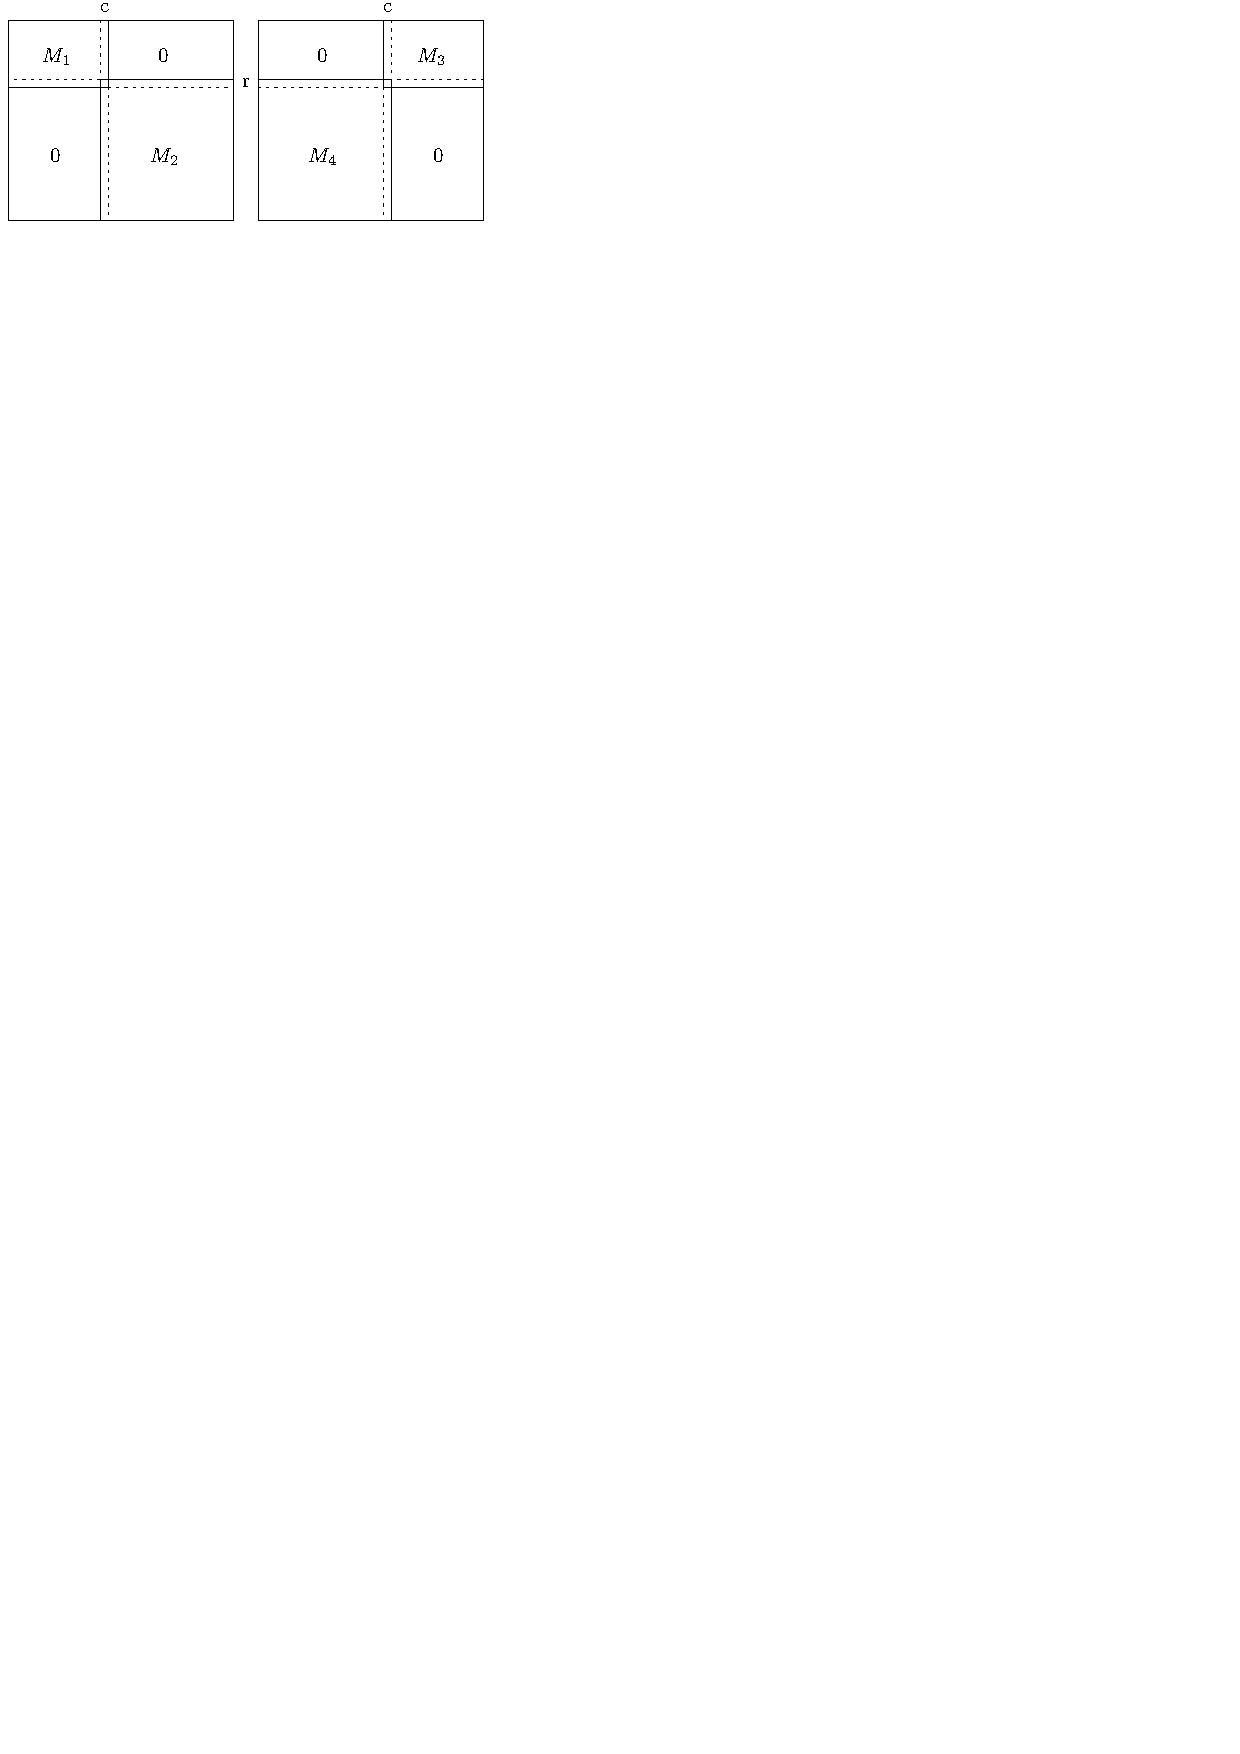
\includegraphics[width=100mm]{img/p33.pdf}
\caption{Characterization of matrices avoiding \usebox{\smlmatb} as an interval minor.}
\label{fig:p33}
\end{figure}
\begin{proof}
\item[$\Rightarrow$] We proceed by induction on the size of $M$.

If $M\in\{0,1\}^{2\times2}$ then it either avoids $\smm{ &\bullet\\\bullet&\bullet}$ or $\smm{\bullet&\bullet\\\bullet& }$ and we are done.

For bigger $M$ there is, from Lemma~\ref{lemma:p33}, $M[r,c]$ satisfying some conditions. If there is a one-entry in any corner, we are done because the matrix cannot contain one of the rotations of $\smm{\bullet&\bullet\\\bullet& }$. Otherwise, assume $M[r,c]$ is both top-right and bottom-left empty and $(r,c)\not\in\{(1,n),(m,1)\}$. If $M_1$ is non-empty, then $\smm{ &\bullet\\\bullet&\bullet}\nim M_2$. Symmetrically, $\smm{\bullet&\bullet\\\bullet& }\nim M_1$ if $M_2$ is non-empty. If one of them is empty, the other is a smaller matrix avoiding $P$ as an interval minor and by induction hypothesis, it can be partitioned.
\item[$\Leftarrow$] Without loss of generality, let us assume $M$ looks like the left matrix in Figure~\ref{fig:p33}. For contradiction, assume $\PimM$. In that case, we can partition $M$ into four quadrants such that there is at least one one-entry in each of them. It does not matter where we partition it, every time we either get $\smm{\bullet&\bullet\\\bullet& }\im M_1$ or $\smm{ &\bullet\\\bullet&\bullet}\im M_2$, which is a contradiction.
\end{proof}

\begin{lemma}
\label{lemma:p72}
For all matrices $M$: $P_8\nim M\Rightarrow M=M_1\rightarrow M_2$ where
\begin{enumerate}
\item $\smm{\bullet&\bullet\\ &\bullet}\nim M_1$ and $\smm{ &\bullet\\\bullet& }\nim M_2$ or
\item $\smm{\bullet& \\ &\bullet}\nim M_1$ and $\smm{\bullet&\bullet\\\bullet& }\nim M_2$.
\end{enumerate}
\end{lemma}
\begin{proof}
Let $e=[r,c]$ be the top-most one-entry of $M$. If $\smm{\bullet&\bullet\\ &\bullet}\im M[[m],[c-1]]$, together with $e$ it would be the whole $P_8$. Symmetrically, $\smm{\bullet&\bullet\\\bullet& }\nim M[[m],[c+1,n]]$. For contradiction assume $\smm{\bullet& \\ &\bullet}\im M[[m],[c]]$ and let $e_{1,1},\ e_{2,2}$ (none of them equal to $e$) be any two one-entries forming the pattern. Symmetrically, assume $\smm{ &\bullet\\\bullet& }\im M[[m],[c,n]]$ and let $e_{1,2},\ e_{2,1}$ be any two one-entries forming the pattern. Then $e_{1,1},\ e,\ e_{1,2}$ and $e_{2,1}$ or $e_{2,2}$ with bigger row give us mapping of $P_8$ to $M$.
\end{proof}

\begin{thm}
For all matrices $M$: $P_8\nim M\Leftrightarrow M$ is structured like the matrix in Figure~\ref{fig:p72} where $\smm{\bullet& \\ &\bullet}\nim M_1$ and $\smm{ &\bullet\\\bullet& }\nim M_2$.
\end{thm}
\begin{figure}[!ht]
\centering
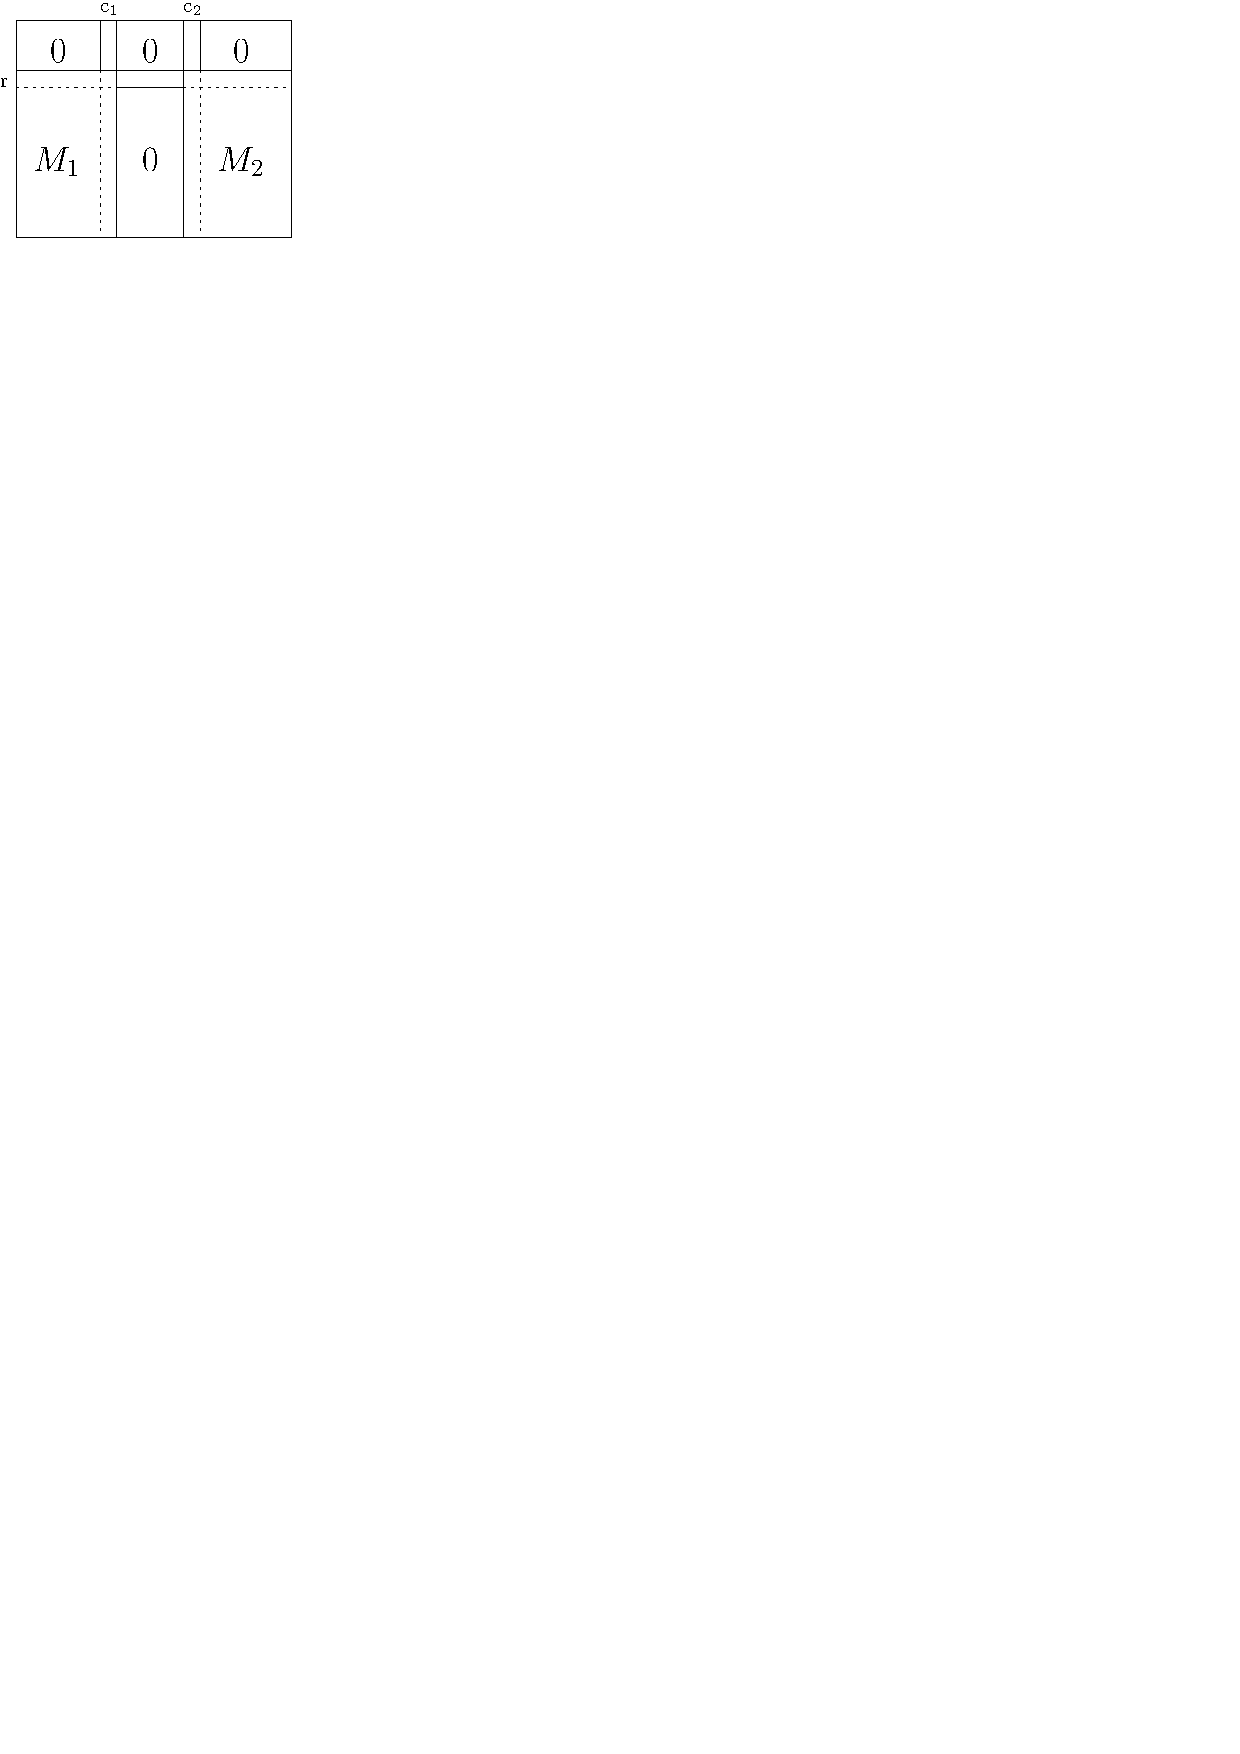
\includegraphics[width=60mm]{img/p72.pdf}
\caption{Characterization of matrices avoiding \usebox{\smlmatc} as an interval minor.}
\label{fig:p72}
\end{figure}
\begin{proof}
\begin{itemize}
	\item[$\Rightarrow$] From Lemma~\ref{lemma:p72} we know $M=M_1'\rightarrow M_2'$ where $\smm{\bullet&\bullet\\ &\bullet}\nim M_1'$ and $\smm{ &\bullet\\\bullet& }\nim M_2'$. The second case can be dealt with symmetrically. From Theorem~\ref{thm:p31} we have that $M_1'$ can be characterized exactly like $M[[m],[c_2-1]$ and $M[[m],[c_2,n]]$ forms a walking matrix. If there are two different columns having a one-entry above the $r$-th row, together with a one-entry in the $r$-th row between the columns $c_1$ and $c_2$ and a one-entry in the $c_1$-th column above the $r$-th row they form a mapping of $P_8$.
	\item[$\Leftarrow$] One-entry $P_8[2,2]$ can not be mapped anywhere but to the $r$-th row, but in that case there are at most two columns having one-entries above it.
\end{itemize}
\end{proof}

\section{Multiple patterns}

\begin{thm}
Let $P_{10}=\smm{\circ&\circ&\bullet\\\bullet&\circ&\circ}$ and $P_{11}=\smm{\circ&\bullet\\\circ&\circ\\\bullet&\circ}$, then for all matrices $M$: $\{P_{10},P_{11}\}\nim M\Leftrightarrow$ for the top-right most walk~$w$ in $M$ such that there are no one-entries underneath it each one-entry $M[r,c]$ is either on $w$ or both $M[r+1,c]$ and $M[r,c-1]$ are on $w$.
\end{thm}
\begin{proof}
\begin{itemize}
	\item[$\Rightarrow$] For contradiction assume there is a one-entry anywhere but on $w$ or directly diagonally above any bottom-left corner of $w$. Then this one-entry together with at least one bottom-left corner of $w$ give us $P_{10}$ or $P_{11}$ and a contradiction.
	\item[$\Leftarrow$] If we take any one-entry~$e$, from the description of $M$ there is no one-entry that creates $P_{10}$ or $P_{11}$ with $e$.
\end{itemize}
\end{proof}